%-----------------------------------------------------------------------------
%
%          PHYSICS  M.S.     THESIS
%          JUSTIN A. VASEL
%
%          This began as the template offered by the University of Minnesota, 
%          but I've made a few changes here and there...  
%
%          -->  halo.tex
%
%-----------------------------------------------------------------------------


\chapter{Helium and Lead Observatory}
	\label{halo_chapter}

	\begin{quoting}
		\noindent \large ``Astronomically Patient" \normalsize

		--- The HALO Collaboration
	\end{quoting}

	\chapterIntro{B}{uried 6,800 feet below ground,} SNOLAB is the deepest laboratory in the world. SNOLAB is located near Sudbury, Ontario, Canada in the Vale Creighton Mine. Originally, the laboratory consisted of just one experiment, the Sudbury Neutrino Observatory (SNO). Due to the success of SNO in shedding light on the solar neutrino problem, the laboratory expanded and now is home to a handful of neutrino and dark matter experiments. The Helium and Lead Observatory (HALO) is one of the experiments that calls SNOLAB its home. 

	The HALO experiment is currently in the final stages of development. When it is complete, HALO will continuously search for the distinct neutrino signal produced during a galactic supernova as a member of SNEWS. HALO is unique in that it is the only neutrino experiment whose primary objective is to detect supernova neutrinos.

	\begin{figure}[H]
		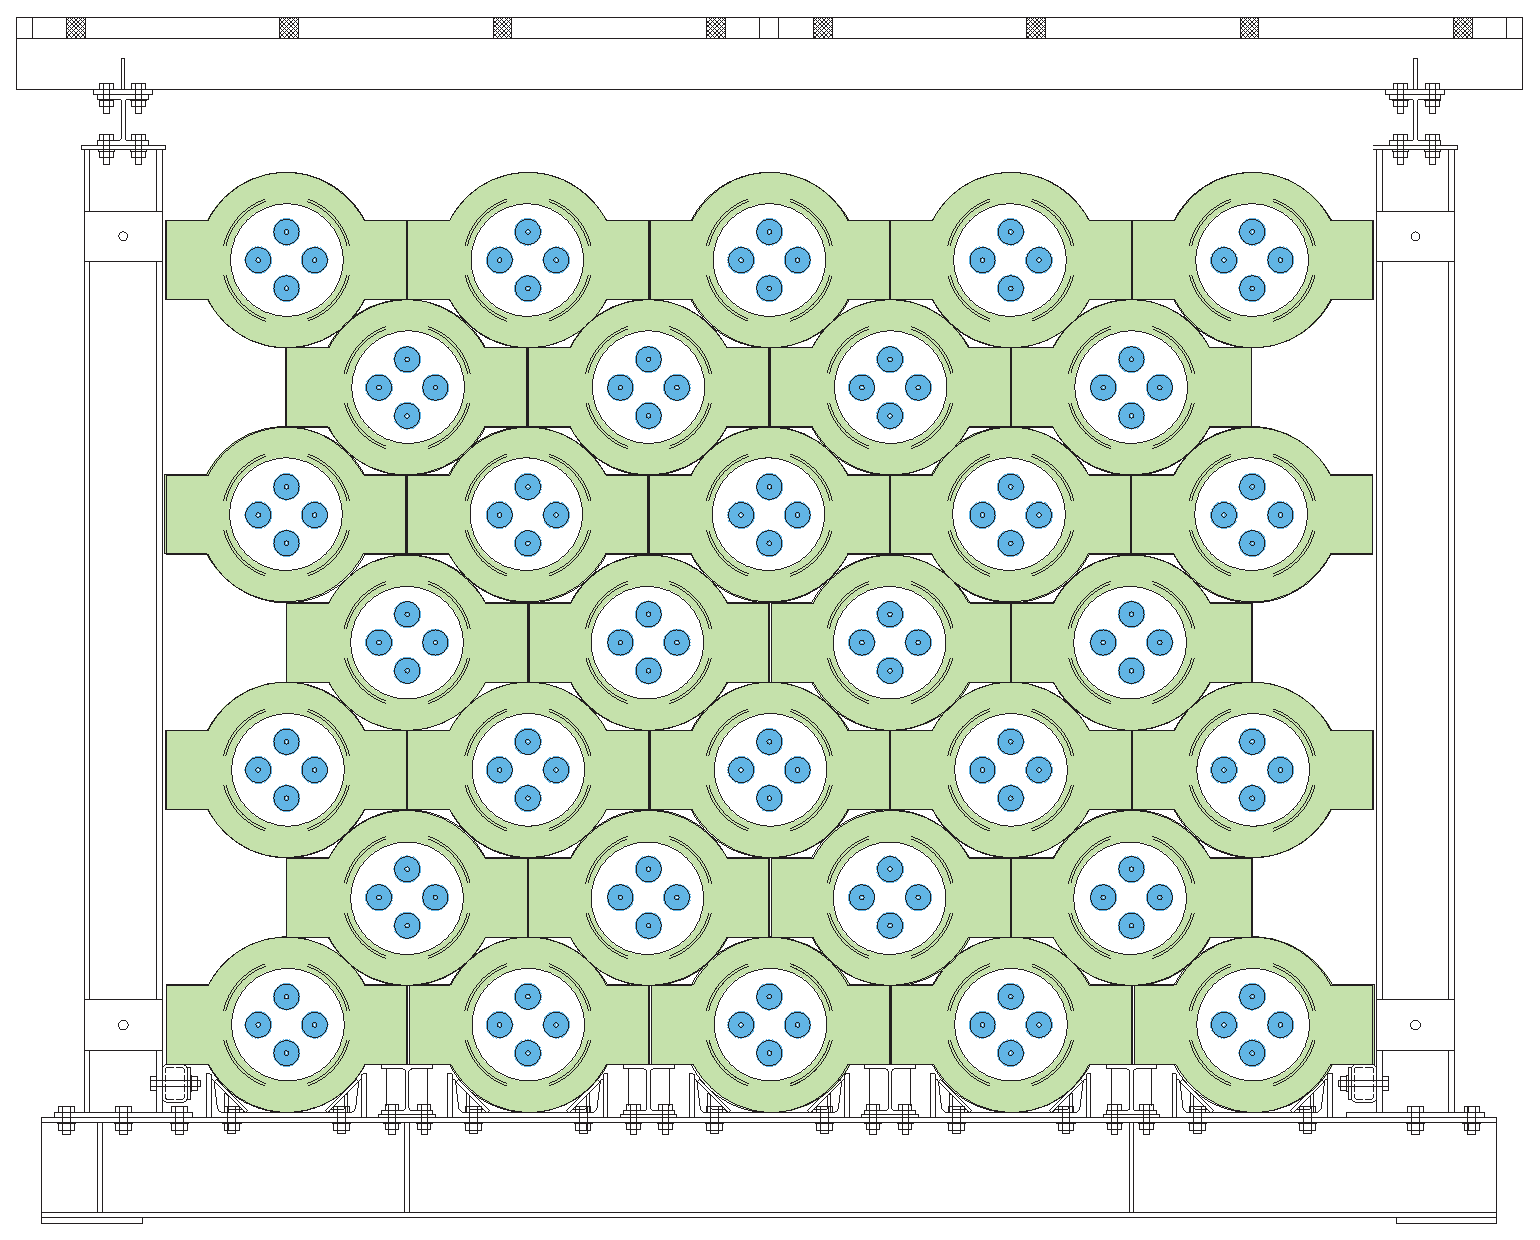
\includegraphics[width=\textwidth]{halo_diagram}
		\caption[The HALO Detector]{\bf Schematic of the HALO detector design (Front View). \rm The lead blocks (stacked objects, shaded green) are the site of neutrino interactions. The products of those interactions, neutrons, travel into the \he proportional counters (four circles contained within each lead block, shaded blue) and are captured on \he. The structure is \SI{2.4}{\metre} tall.}
		\label{fig:halo}
	\end{figure}

	The HALO detector consists of \ \SI[mode=text]{76}{tons} of lead and 128 \he neutron detectors. The lead serves as the interaction medium and is sectioned in blocks. Each block of lead has a bore through the middle of it within which sit four \he neutron detectors \nolinebreak (\FIG \ref{fig:halo}). The 864 lead blocks used in HALO are stacked in such a way that every bore extends \SI{3}{\metre} in length. Most of the \he detectors are also \SI{3}{\metre} long. However, there were not enough detectors of that length to fill up all 128 positions. Several \SI{2.5}{\metre} long detectors were used to fill the extra space.

	Because galactic supernovae only occur two or three times each century\footnote{Despite this predicted occurrence rate, the most recently observed supernova within the Milky Way was spotted by Johannes Kepler in 1604.}\cite{sn_rates}, HALO is designed with longevity in mind. Once completed, the experiment will be highly automated and relatively inexpensive to maintain, allowing it to remain in operation for decades. 



	%% SECTION : LEAD AS AN INTERACTION MEDIUM
	\section{Lead as a Interaction Medium}

	HALO is the only neutrino experiment that uses lead as an interaction medium. Lead was chosen because it was economical, available, and efficiently delivers neutrino-induced neutrons to the \he neutron counters in which detection actually occurs. Lead has a relatively high neutrino interaction cross section which results in the production of neutrons\cite{Engel2003}. These interactions (\FIG \ref{fig:sensitivities}) are neutral current (NC) interactions, which are moderated by the $\HepParticle{\PZzero}{}{}$ boson (\EQ \ref{eq:nc}), or charged current (CC) interactions, which are moderated by the $\HepParticle{\PWpm}{}{}$ bosons (\EQS \nolinebreak \ref{eq:nue_cc} \& \nolinebreak \ref{eq:nue_bar_cc}).
		\begin{align}
			\quad \textbf{Neutral Current} \qquad &\HepProcess{\HepParticle{\Pneutrino}{}{} + \text{Pb} \to \HepParticle{\Pneutrino}{}{*} + \text{Pb}^*} \label{eq:nc} \\
			\quad \textbf{$\HepParticle{\Pnue}{}{}$ Charged Current} \qquad &\HepProcess{\HepParticle{\Pnue}{}{} + \text{Pb} \to \HepParticle{\Pelectron}{}{} + \text{Bi}^*} \label{eq:nue_cc} \\
			\quad \textbf{$\HepParticle{\APnue}{}{}$ Charged Current} \qquad &\HepProcess{\HepParticle{\Pnue}{}{} + \HepParticle{\Pproton}{}{} \to \HepParticle{\Ppositron}{}{} + \HepParticle{\Pneutron}{}{}} \label{eq:nue_bar_cc}
		\end{align}
		In NC interactions, a neutrino of any flavor strikes a lead nucleus and excites it. When the nucleus de-excites, zero, one, or two neutrons are produced ($\HepProcess{\text{Pb}^* \to \text{Pb} + \HepParticle{\Pphoton}{}{} + \text{neutrons}}$). In $\HepParticle{\Pnue}{}{}$ CC interactions, an electron neutrino interacts with a neutron in the lead nucleus, producing an electron and bismuth in an excited state. Again, the nucleus de-excites and produces zero, one, or two neutrons ($\HepProcess{\text{Bi}^* \to \text{Bi} + \HepParticle{\Pphoton}{}{} + \text{neutrons}}$).

		\begin{figure}[H]
			
\includegraphics[width=\textwidth]{total}
			\vspace{-0.3in}
			\caption[Neutrino Detector Sensitivities]{\bf Neutrino detector sensitivities. \rm Different neutrino interaction materials have different neutrino flavor sensitivities. This figure shows which interaction channels appear as a proportion of the total neutrino signal for popular interaction media. Since HALO is the first experiment to lead as an interaction medium, it will offer unique insight into the $\HepParticle{\Pnue}{}{}$ charged current channel.}
			\label{fig:sensitivities}
		\end{figure}
		\vspace{-0.1in}
	Scaling from the calculations of Engel, McLaughlin, and Volpe\cite{Engel2003}, a supernova \SI{10}{\kilo\parsec} from Earth would produce 29 single neutrons and 18 double neutrons from the charged current channel, and 8 single neutrons and 6 double neutrons from the neutral current channel\cite{Shantz2010}. Not all of these events will be detected, however. HALO's detection efficiency is estimated to be $\sim 40\%$\cite{Shantz2010,Scholberg2011}. The efficiency will be more accurately known after improvements have been made to the detector Monte Carlo simulation.

	The third possible interaction, $\HepParticle{\APnue}{}{}$ CC, is highly suppressed due to ``Pauli blocking.'' The excess of neutrons in lead makes it less likely that neutron will be produced because many of the low-energy states are already filled, and neutrons are fermionic particles that are subject to the Pauli exclusion principle. 

	The lead blocks were originally used in the Deep River cosmic ray monitoring station\cite{Shantz2010}. The lead is stacked in alternating rows of four and five (\FIG \ref{fig:halo}) and each row runs 3 meters deep. This geometry was chosen to maximize the number of lead blocks used while being confined to the relatively small space that HALO is given in SNOLAB. HALO makes use of 76 tons of lead; 864 blocks in total. The lead blocks were painted to minimize health risks associated with exposure to lead and to minimize contamination of the SNOLAB environment. The paint was meticulously chosen based on several factors, including its resistance to peel or rust, its neutron-capture cross section, and its containment of radioactive isotopes that could increase background noise in the detector\cite{Shantz2010}.



	%% SECTION : 3HE PROPORTIONAL COUNTERS
	\section{\he Proportional Counters}

	\begin{figure}[H]
		\includegraphics[width=\textwidth]{ncd}
		\caption[Technical Diagram of \he Proportional Counter]{\bf Technical diagram of \he proportional counter\rm \cite{Schumaker2010}. The counters were originally used in Phase III of the SNO experiment, but have been refitted with new endcaps for use in HALO.}
		\label{fig:ncd}
	\end{figure}

	The neutrons produced from nuclear de-excitation of either lead or bismuth pass into one of the 128 proportional detectors (\FIG \ref{fig:ncd}) which are filled with a gaseous mixture of \he and CF$_4$ (85/15 by pressure) at a pressure of \SI[mode=text]{2.5}{atm}. The neutrons are captured on \he shortly after entering the tube by the following reaction:
	\begin{equation}
		\HepProcess{^3\text{He} + \HepParticle{\Pneutron}{}{} \to \HepParticle{\Pproton}{}{} + {}^3\text{H} + \ekeV{764}}
	\end{equation}
	Of the \ekeV{764} released from the reaction, \ekeV{573} is the kinetic energy of the proton and \ekeV{191} is the kinetic energy of the triton. The production of these charged particles (\FIG \ref{fig:capture}) ionizes the nearby gas, producing ion pairs that are accelerated in opposite directions by a potential difference between a coaxial anode and cathode. The electric field near the anode is strong enough to allow secondary ionization of the surrounding gas by the accelerating electrons. This produces a cascade of ionization that is ultimately collected on the anode. The amount of charge collected at the anode is proportional to the original number of ion pairs. 

	\begin{figure}[H]
		\centering
		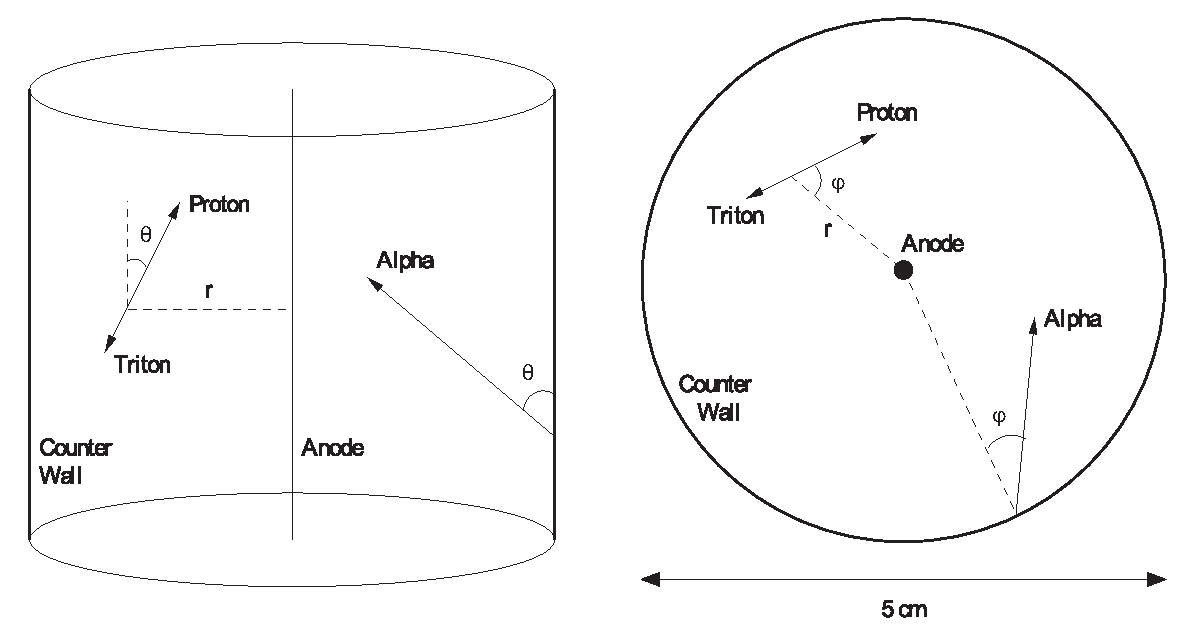
\includegraphics[width=0.9\textwidth]{capture}
		\caption[\he Neutron Capture Schematic]{\bf \he Neutron capture schematic\rm \cite{Search2011}. The proton-triton pair are produced and move in opposite directions. The proton and triton peaks may be separated in time by an amount determined by their orientation in the counter.}
		\label{fig:capture}
	\end{figure}

	The spectrum of neutron energies does not have a single sharp peak at \ekeV{764}, however. Instead, the spectrum has two distinct shoulders to the left of the peak (\FIG \nolinebreak \ref{fig:neutron_spectrum}). These shoulders are artifacts of the ``wall effect.'' The wall effect occurs when neutron capture happens very close to the detector wall. When the proton and triton are created, one of them may collide with the wall of the detector or be absorbed by it entirely, reducing the total kinetic energy detected by the counter.

	\begin{figure}[H]
		\centering
		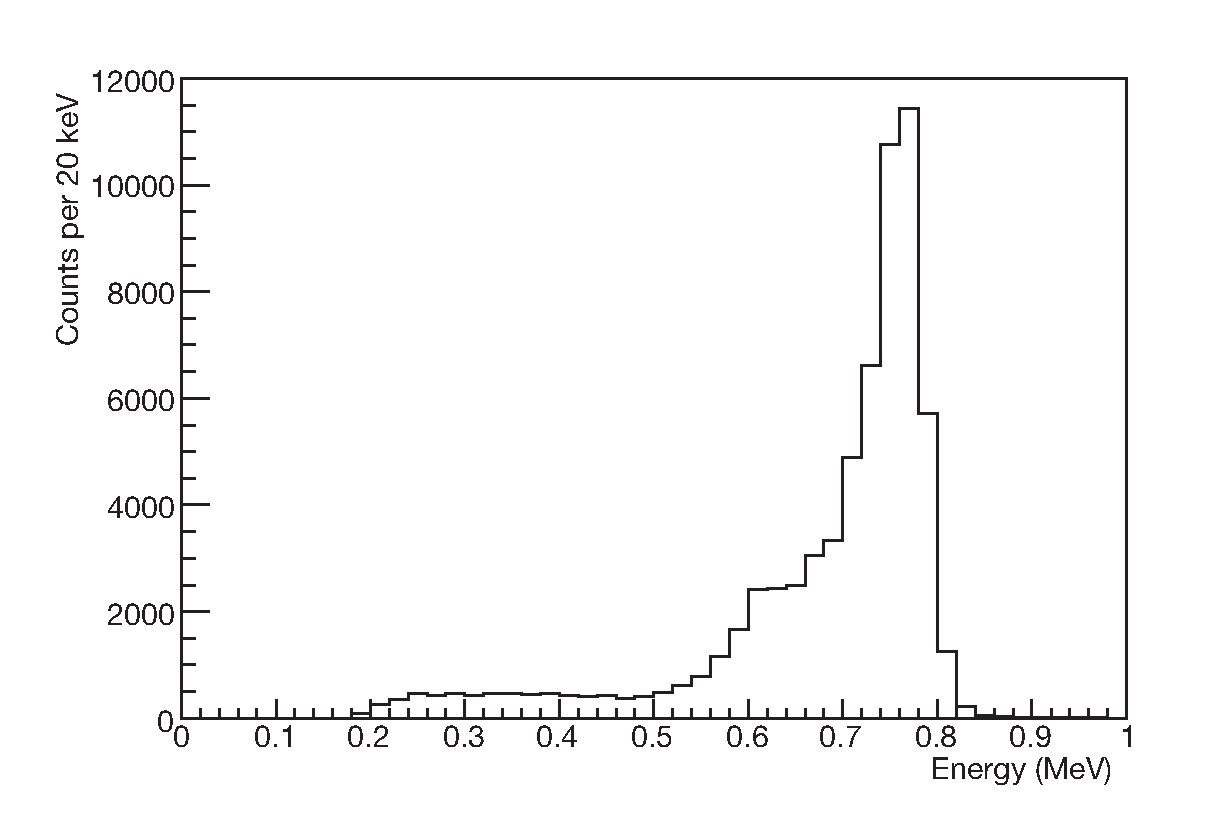
\includegraphics[width=0.9\textwidth]{neutron_spectrum}
		\caption[Example Neutron-Capture Spectrum]{\bf \he neutron-capture spectrum from $^{24}$Na calibration\rm \cite{Search2011}. The neutron peak is clearly located at \ekeV{764}, but there also exist shoulders that terminate at \ekeV{573} and \ekeV{191} due to some of the triton's or proton's energy (respectively) being lost due to collisions with the walls of the counter.}
		\label{fig:neutron_spectrum}
	\end{figure}


	%% SECTION : NEUTRON BACKGROUNDS AND NOISE
	\section{Neutron Backgrounds and Noise}
	\label{sec:noise}
	SNOLAB is better than any other laboratory when it comes to shielding. The \SI[mode=text]{6800}{feet} of rock that sit above it is the equivalent of \SI{6000}{\meter} of water. That notwithstanding, there is still background flux of both fast and thermal neutrons produced by radioactive decays and cosmic ray muon interactions within the surround rock. The flux of thermal and fast neutrons in SNOLAB has been measured to be \SI[mode=text]{4100}{neutrons.m^{-2}.day^{-1}} and \SI[mode=text]{4000}{neutrons.m^{-2}.day^{-1}} respectively\cite{handbook}. 

	To ensure that HALO will maintain the false-alarm rate required for participation in SNEWS (see \SEC \ref{sec:snews_positive}), shielding has been placed around the detector to block as much of the neutron background as possible. Hydrogen makes a great neutron shield because its small mass makes it effective at stealing momentum from fast neutrons, slowing them down. Capture of the thermal neutrons by hydrogen can then occur. The shielding is in the form of water boxes that have a volume of \SI[mode=text]{1}{ft^3}. The boxes have a bladder inside to hold the water. The empty spaces in the box that are not occupied by the water bladder are filled with polystyrene beads. These boxes are placed along the top, back, and sides of the detector. Soon water boxes will cover up the front face of the detector as well.
 
	The proportional counters are very effective as long as ionization is induced by neutron capture events only. Collisions within\he gas can excite molecules without ionizing them, leading to the emission of a photon when the molecule de-excites. The photons can then go on to cause ionization elsewhere in the detector. This is the reason for the \he/CF$_4$ mixture. The CF$_4$ provides stopping power for ionizing particles, substantially reducing the effect.

	The outer shell of the\he counter is composed of ultra-pure nickel. The walls are only \SI{380}{\micron} thick and were produced in a uniform way through the process of chemical vapor deposition. Despite the purity of the detector material, there are trace amounts of radioactive nuclei that contribute to noise in the signal. The most common byproduct of radioactive decays are alpha particles. The alphas can interact with other elements resulting in the production of a neutron. Fortunately, alpha particles have charge and are very heavy, so they have a very short range. This prevents them in many cases from arriving at the detector wall with sufficient energy to initiate radioactive decay. 

	The few neutrons that are produced by interactions with alpha particles have energies that are a couple tens of \eMeV{}, making them indistinguishable from neutrons produced by supernova neutrino interactions. A study of these alpha backgrounds found that the rate of neutron-producing alphas was $21.9^{+1.1}_{-1.0}$ per day and is considered negligible \cite{Shantz2010}. 

	Gamma rays are another source of noise and are produced through nuclear decays of uranium and thorium found in the paint that coats the lead blocks. Uranium and thorium decay via $\alpha$ or $\beta$ emission, but the decay of daughter nuclei can produce gammas. The gammas then can interact with electrons via Compton scattering and induce ionization within the \he detectors. Multiple scattering effects may imbue the electrons with enough energy to survive being cut by detector electronics, resulting in the false count of a neutron. Simulations\cite{Shantz2010} and HALO data show that the energy of these gamma-induced counts tends to be less than a few \eMeV{}, making them easily distinguishable from the neutrino-induced neutron signal.

 	%% SECTION : DETECTOR ELECTRONICS AND DATA FLOW
	\section{Detector Electronics and Data Acquisition}
	\label{sec:electronics}
		The HALO detector and its associated hardware is controlled by a software application called ORCA. This software will be described in greater detail in \SEC \ref{sec:orca_development}. For now, I will briefly describe the electronics configuration of the experiment. The flow of data is illustrated in \FIG \ref{fig:electronics}. The charge collected by the \he counter anode is converted into a voltage and stepped up to a higher voltage by a preamplifier (preamp). The 128 detectors are connected in pairs, so only 64 preamps are used. The signal from the preamps is read into one of 8 shaper ADC boards, each having 8 channels. The shaper ADCs discriminate the signal according to thresholds that are set by the experimenters and then digitize the signal.

		The shaper cards then pass the digitized signal to a single board computer (SBC) running Linux through a common VME bus. The SBC then passes the data to the ORCA software running on the DAQ computer. The HV on the preamps is controlled through ORCA. A HV feedback ADC is used to continuously monitor the voltage. 

		A pulse distribution system has been implemented recently (not shown in \FIG \ref{fig:electronics}). The system allows experimenters to send a simulated pulse into the preamps as a means of testing their response. The system can also be used to characterize the response of the detector. For example, the pulser was recently used to measure the time delay between the recording of events that occurred in separate detectors simultaneously\cite{pulser_timing}. Pulses are timestamped by the trigger card. Currently, the times are provided by an NTP (Network Time Protocol) server on a local Linux box. To produce more accurate timestamps, the collaboration is currently working with SNOLAB to acquire GPS NTP servers. 
		\begin{figure}[H]
			\includegraphics[width=\textwidth]{electronics}
			\caption[HALO Electronics]{\bf HALO electronics diagram. \rm The \he detectors are joined in pairs and connected to 64 preamps where the charge collected at the \he counter anode is converted into a high voltage (HV). The signal is sent to shaper ADC boards which digitize and integrate the current. The digitized signal is then sent to a Linux single board computer (SBC) and is passed to the ORCA software that runs on the DAQ computer. The HV system is controlled by the ORCA software. A HV ADC is used as a feedback mechanism to monitor the voltages in nearly-real-time. A pulse distribution (not shown) has been implemented to allow the injection of simulated pulse signals into the preamps as a way to test their response.}
			\label{fig:electronics}
		\end{figure}


%-----------------------------------------------------------------------------
%-----------------------------------------------------------------------------